\section{Theorie}
\label{sec:Theorie}

Wird die Ausbreitung von Lichtstrahlen durch Hindernisse beeinflusst, so kann die Ablenkung dieser anhand der geometrischen 
Optik beschrieben werden. In dem Spezialfall, dass Licht eine Öffnung in einem Schirm, die kleiner als der Durchmesser des 
Lichtstrahls ist, durchquert, so lässt sich die Ablenkung über das Huygenssche Prinzip beschreiben. Dabei wird ausschließlich 
der Wellencharakter des Lichts berücksichtigt, was bei hinreichend großer Lichtquantenanzahl, über die gemittelt werden kann, 
ausreichend ist. Über eine Fourier-Transformation können die Funktionen des beugenden Objektes und die der winkelabhängigen 
Intensitätsverteilung des Lichts ineinander überführt werden. Im vorliegenden Versuch beschränkt sich die Untersuchung
auf einen parallelen Einzelspalt, an dem das Licht gebeugt wird. 

Es wird dabei allgemein zwischen zwei Arten der Beugung, der Fresnelschen und der Fraunhoferschen Beugung, unterschieden.
Bei der Fresnelschen Beugung ist der Abstand zwischen Quelle und Spalt, wie auch zwischen Spalt und Beobachtungsschirm endlich,
sodass die Lichtstrahlen mit verschiedenen Winkeln den Spalt durchqueren und dadurch unterschiedliche Beugungswinkel erfahren, 
wodurch sich eine Interferenz auf dem Beobachtungsschirm ergibt. Die Fraunhofersche Beugung setzt die Näherung vorraus, dass 
sowohl der Abstand von Quelle zu Spalt, als auch von Spalt zu Schirm unendlich ist, was z.B. mittels einer Sammellinse simuliert
werden kann. Die Lichtstrahlen treffen also alle mit dem gleichen Beugungswinkel auf den Schirm auf. In der 
Abbildung \ref{fig:strahlen} sind die schematischen Strahlenverläufe der beiden beschriebenen Beugungsarten dargestellt. 
\begin{figure}
    \centering
    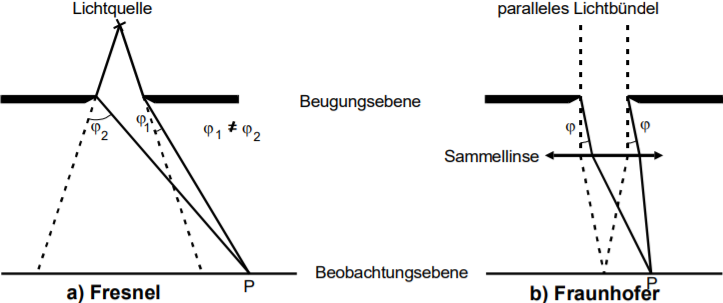
\includegraphics[width=\textwidth]{data/fres_fraun.png}
    \caption{Schematische Darstellung der Strahlenverläufe bei Fresnel und Fraunhofer Beugung}
    \label{fig:strahlen}
\end{figure}

Im Folgenden wird nur die Fraunhofersche Beugung betrachtet, da mit dieser im Versuch gearbeitet wird. 
In der Abbildung \ref{fig:strahlen} ist schematisch der Verlauf des Lichts nach der Beugung am Spalt gezeigt. Nach der Beugung einer 
ebenen Welle mit der Feldstärke
\begin{equation}
    A(z,t) = A_0 e^{i(\omega t - 2\pi z / \lambda)} 
\end{equation}
breiten sich von jedem Punkt der Wellenfront nach dem Huygensschen Prinzip Elementarwellen mit Kugelform aus. Diese Wellen 
überlagern sich und erzeugen so eine neue Wellenfront, die der Einhüllenden der Elementarwellen entspricht. Der Phasenunterschied
zwischen zwei Strahlenbündeln, die den Abstand $x$ zueinander haben, kann durch 
\begin{equation}
    \delta = \frac{2\pi x \sin \phi}{\lambda}
\end{equation}
beschrieben werden. Wird der Abstand $x$  als infinitisimal angesehen, so kann für die Funktion der Amplitude $B$ über die gesamte
Spaltbreite $b$  integriert werden, wodurch die Gleichung 
\begin{align}
    B(z,t,\varphi) &= A_0 \int_0^b \mathrm{e}^{i(\omega t - \frac{2 \pi z}{\lambda} + \delta)} \mathrm{d}x \\
    &= A_0 \mathrm{e}^{i \left (\omega t - \frac{2 \pi z}{\lambda} \right )} \cdot \mathrm{e}^{\frac{\pi i b \sin \varphi}{\lambda}} \cdot \frac{\lambda}{\pi \sin \varphi} \cdot \sin \left (\frac{\pi b \sin \varphi}{\lambda} \right )
   \label{eqn:amp}
\end{align}
entsteht. 
Die beiden Expenonentialterme sind für die Intensitätsverteilung unwichtig. Wird 
\begin{equation}
    \eta := \frac{\pi b \sin\phi}{\lambda}
\end{equation}
definiert, so lässt sich $B(\phi)$ als 
\begin{equation}
    B(\phi) = A_0 b \frac{\sin\eta}{\eta}
    \label{eqn:amp_ez}
\end{equation}
ausdrücken. Die Gestalt dieser Funktion ist in Abb \ref{fig:int_vert} dargestellt, wobei die Nullstellen der Funktion an den Stellen
\begin{equation}
    \sin \phi_n = \pm n\frac{\lambda}{b}\;\text{mit}\; n\in \mathds{N}
\end{equation} 
sind. Eine direkte Messung der Amplituden der Lichtwelle ist aufgrund der hohen Frequenz mit dem vorliegenden Aufbau nicht möglich,
weshalb auf eine Messung der zeitlich gemittelten Intensität zurückgegriffen wird, die durch 
\begin{equation}
    I(\phi) = B(\phi)^2 = A_0^2 b^2 \Biggl(\frac{\lambda}{\pi b \sin\phi}\Biggr)^2 \cdot \sin^2\Biggl(\frac{\pi b\sin\phi}{\lambda}\Biggr)
    \label{eqn:aus}
\end{equation}
beschrieben wird. Dabei befinden sich die Minima an den Nullstellen der Gleichung \ref{eqn:amp_ez} und die Maxima nehmen näherungsweise 
mit dem Quadrat des Beugungswinkels ab. 
\begin{figure}
    \centering
    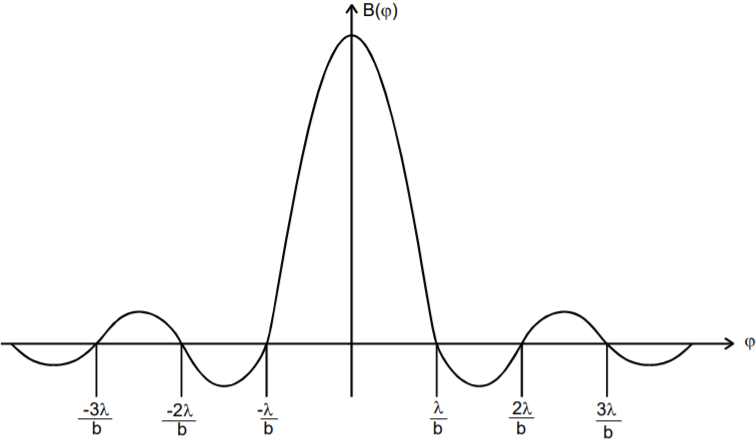
\includegraphics[width=\textwidth]{data/amp_verteilung.png}
    \caption{Verteilung der Amplituden der Beugungsfunktion bei Beugung an einem Parallelspalt.}
    \label{fig:int_vert}
\end{figure}

Die Amplitudenfunktion $B(\phi)$ kann auch als Fourier-Transformierte der einfallenden Wellenfunktion beschrieben werden. 
Die allgemeine Form einer Fourier-Transformation der Funktion $f(x) $ ist 
\begin{equation}
    g(\xi) := \int_{-\infty}^\infty f(x)\mathrm{e}^{i x \xi} \mathrm{d}x\,.
\end{equation}
Mit der Aperturfunktion 
\begin{align}
    f(x) &= A_0\,,& 0\leq x\leq b\\
    f(x) &= 0\,,& sonst 
\end{align}
ergibt sich dann über weitere Umformungen
\begin{equation}
    g(\xi) = \frac{2A_0}{\xi} \mathrm{e}^{\Bigl(\frac{i\xi b}{2}\Bigr)}\cdot\sin\frac{\xi b}{2}\,.
\end{equation}
Dies entspricht der Gleichung \ref{eqn:amp}, wenn 
\begin{equation}
    \xi := \frac{2\pi\sin\phi}{\lambda}
\end{equation}
ist.

Damit ist eine mathematische Beschreibung des Huygensschen Prinzips gegeben. Die Fourier-Transformation ist invertierbar, wodurch aus der 
Intensitätsverteilung der gebeugten Lichtwellen rückschließend die Form des beugenden Objekts bestimmt werden kann. 